\documentclass{standalone}
\usepackage{tikz}
\usetikzlibrary{patterns, positioning}

\begin{document}
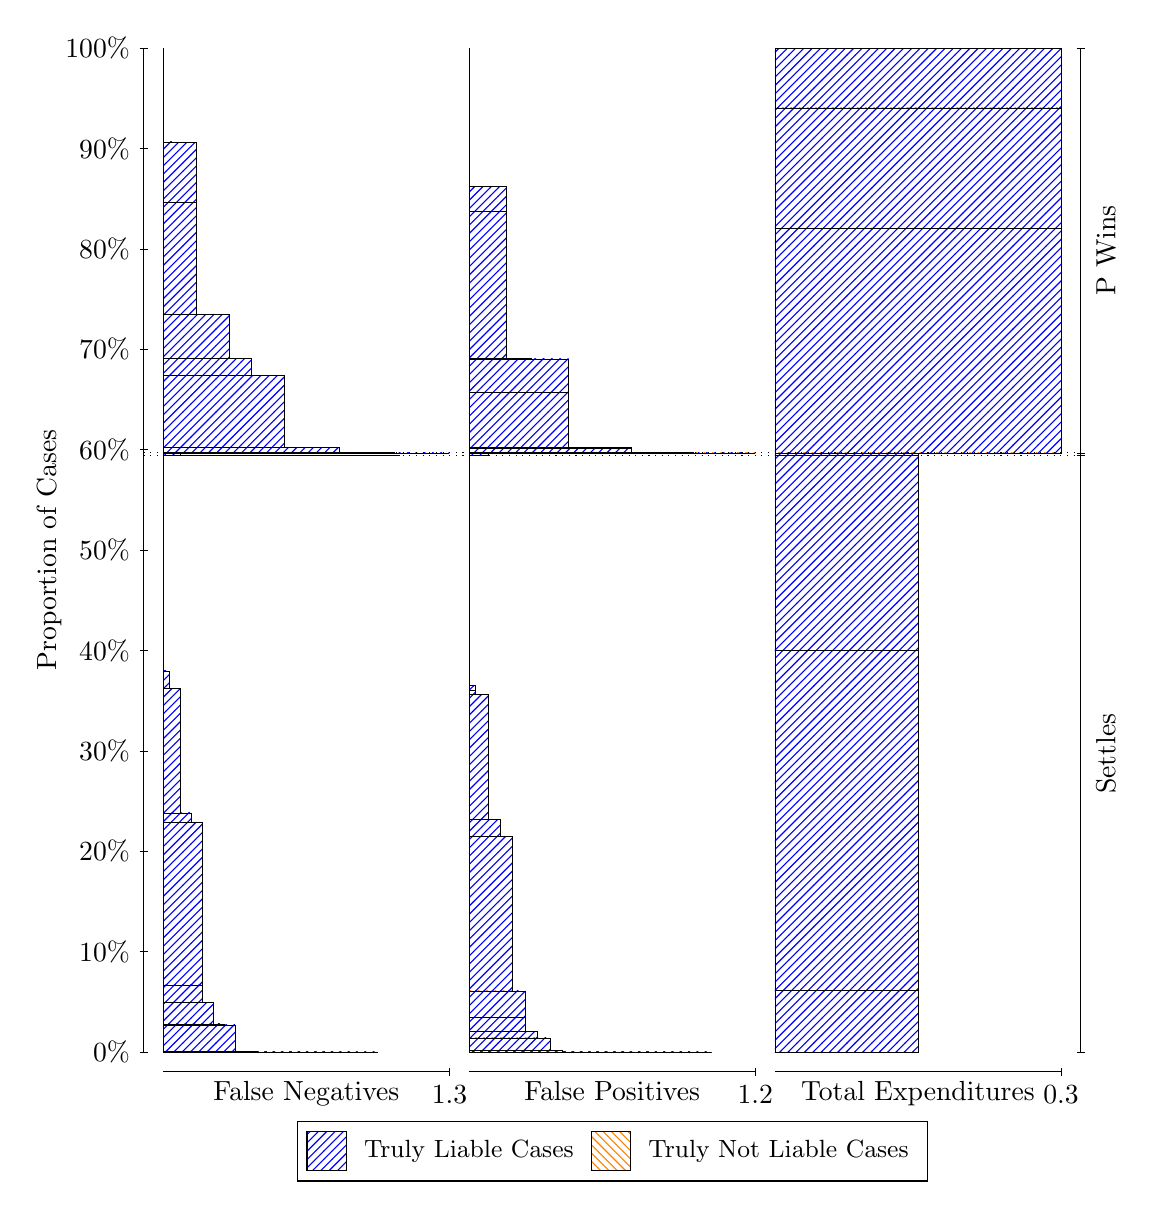
\begin{tikzpicture}
\draw[black, very thin] (1.5,1.75) -- (1.5,14.5);
\node[rotate=90, anchor=center] at (0.3, 8.125) {Proportion of Cases};
\draw[black, very thin] (1.45,1.75) -- (1.55,1.75);
\node[anchor=east] at (1.45, 1.75) {0\%};
\draw[black, very thin] (1.45,3.025) -- (1.55,3.025);
\node[anchor=east] at (1.45, 3.025) {10\%};
\draw[black, very thin] (1.45,4.3) -- (1.55,4.3);
\node[anchor=east] at (1.45, 4.3) {20\%};
\draw[black, very thin] (1.45,5.575) -- (1.55,5.575);
\node[anchor=east] at (1.45, 5.575) {30\%};
\draw[black, very thin] (1.45,6.85) -- (1.55,6.85);
\node[anchor=east] at (1.45, 6.85) {40\%};
\draw[black, very thin] (1.45,8.125) -- (1.55,8.125);
\node[anchor=east] at (1.45, 8.125) {50\%};
\draw[black, very thin] (1.45,9.4) -- (1.55,9.4);
\node[anchor=east] at (1.45, 9.4) {60\%};
\draw[black, very thin] (1.45,10.675) -- (1.55,10.675);
\node[anchor=east] at (1.45, 10.675) {70\%};
\draw[black, very thin] (1.45,11.95) -- (1.55,11.95);
\node[anchor=east] at (1.45, 11.95) {80\%};
\draw[black, very thin] (1.45,13.225) -- (1.55,13.225);
\node[anchor=east] at (1.45, 13.225) {90\%};
\draw[black, very thin] (1.45,14.5) -- (1.55,14.5);
\node[anchor=east] at (1.45, 14.5) {100\%};

\draw[black, very thin] (13.4,1.75) -- (13.4,14.5);
\draw[black, very thin] (13.35,1.75) -- (13.45,1.75);
\node[anchor=west] at (13.35, 1.75) {};
\draw[black, very thin] (13.35,9.3238) -- (13.45,9.3238);
\node[anchor=west] at (13.35, 9.3238) {};
\draw[black, very thin] (13.35,9.3588) -- (13.45,9.3588);
\node[anchor=west] at (13.35, 9.3588) {};
\draw[black, very thin] (13.35,14.5) -- (13.45,14.5);
\node[anchor=west] at (13.35, 14.5) {};

\draw[black, very thin, pattern color=blue, pattern=north east lines] (1.75,1.75) rectangle (4.475,1.75);
\draw[black, very thin, pattern color=blue, pattern=north east lines] (1.75,1.75) rectangle (4.1955,1.75);
\draw[black, very thin, pattern color=blue, pattern=north east lines] (1.75,1.75) rectangle (3.916,1.75);
\draw[black, very thin, pattern color=blue, pattern=north east lines] (1.75,1.75) rectangle (3.7763,1.75);
\draw[black, very thin, pattern color=blue, pattern=north east lines] (1.75,1.75) rectangle (3.6365,1.75);
\draw[black, very thin, pattern color=blue, pattern=north east lines] (1.75,1.75) rectangle (3.4968,1.75);
\draw[black, very thin, pattern color=blue, pattern=north east lines] (1.75,1.75) rectangle (3.3571,1.7508);
\draw[black, very thin, pattern color=blue, pattern=north east lines] (1.75,1.7508) rectangle (3.2173,1.7508);
\draw[black, very thin, pattern color=blue, pattern=north east lines] (1.75,1.7508) rectangle (3.0776,1.7512);
\draw[black, very thin, pattern color=blue, pattern=north east lines] (1.75,1.7512) rectangle (2.9378,1.7531);
\draw[black, very thin, pattern color=blue, pattern=north east lines] (1.75,1.7531) rectangle (2.7981,1.7565);
\draw[black, very thin, pattern color=blue, pattern=north east lines] (1.75,1.7565) rectangle (2.6583,2.0954);
\draw[black, very thin, pattern color=blue, pattern=north east lines] (1.75,2.0954) rectangle (2.5186,2.1066);
\draw[black, very thin, pattern color=blue, pattern=north east lines] (1.75,2.1066) rectangle (2.5186,2.1066);
\draw[black, very thin, pattern color=blue, pattern=north east lines] (1.75,2.1066) rectangle (2.3788,2.3841);
\draw[black, very thin, pattern color=blue, pattern=north east lines] (1.75,2.3841) rectangle (2.2391,2.6007);
\draw[black, very thin, pattern color=blue, pattern=north east lines] (1.75,2.6007) rectangle (2.2391,4.6664);
\draw[black, very thin, pattern color=blue, pattern=north east lines] (1.75,4.6664) rectangle (2.0994,4.7857);
\draw[black, very thin, pattern color=blue, pattern=north east lines] (1.75,4.7857) rectangle (1.9596,6.3685);
\draw[black, very thin, pattern color=blue, pattern=north east lines] (1.75,6.3685) rectangle (1.8199,6.5894);
\draw[black, very thin, pattern color=blue, pattern=north east lines] (1.75,6.5894) rectangle (1.8199,6.5894);
\draw[black, very thin, pattern color=orange, pattern=north west lines] (1.75,6.5894) rectangle (1.75,6.5894);
\draw[black, very thin, pattern color=blue, pattern=north east lines] (1.75,6.5894) rectangle (1.75,9.3238);
\draw[black, very thin, pattern color=blue, pattern=north east lines] (1.75,9.3238) rectangle (4.7545,9.3238);
\draw[black, very thin, pattern color=blue, pattern=north east lines] (1.75,9.3238) rectangle (4.0558,9.3238);
\draw[black, very thin, pattern color=blue, pattern=north east lines] (1.75,9.3238) rectangle (3.3571,9.3239);
\draw[black, very thin, pattern color=blue, pattern=north east lines] (1.75,9.3239) rectangle (2.6583,9.329);
\draw[black, very thin, pattern color=blue, pattern=north east lines] (1.75,9.329) rectangle (1.9596,9.3588);
\draw[black, very thin, pattern color=orange, pattern=north west lines] (1.75,9.3588) rectangle (1.75,9.3588);
\draw[black, very thin, pattern color=blue, pattern=north east lines] (1.75,9.3588) rectangle (5.3833,9.3588);
\draw[black, very thin, pattern color=blue, pattern=north east lines] (1.75,9.3588) rectangle (4.6846,9.3598);
\draw[black, very thin, pattern color=blue, pattern=north east lines] (1.75,9.3598) rectangle (4.2654,9.3598);
\draw[black, very thin, pattern color=blue, pattern=north east lines] (1.75,9.3598) rectangle (3.9859,9.4318);
\draw[black, very thin, pattern color=blue, pattern=north east lines] (1.75,9.4318) rectangle (3.5667,9.4319);
\draw[black, very thin, pattern color=blue, pattern=north east lines] (1.75,9.4319) rectangle (3.2872,10.339);
\draw[black, very thin, pattern color=blue, pattern=north east lines] (1.75,10.339) rectangle (2.8679,10.561);
\draw[black, very thin, pattern color=blue, pattern=north east lines] (1.75,10.561) rectangle (2.5885,11.113);
\draw[black, very thin, pattern color=blue, pattern=north east lines] (1.75,11.113) rectangle (2.1692,12.543);
\draw[black, very thin, pattern color=blue, pattern=north east lines] (1.75,12.543) rectangle (2.1692,13.305);
\draw[black, very thin, pattern color=blue, pattern=north east lines] (1.75,13.305) rectangle (1.8897,13.307);
\draw[black, very thin, pattern color=orange, pattern=north west lines] (1.75,13.307) rectangle (1.75,13.307);
\draw[black, very thin, pattern color=blue, pattern=north east lines] (1.75,13.307) rectangle (1.75,14.5);
\draw[black, very thin, pattern color=orange, pattern=north west lines] (5.6333,1.75) rectangle (8.7138,1.75);
\draw[black, very thin, pattern color=blue, pattern=north east lines] (5.6333,1.75) rectangle (8.7138,1.75);
\draw[black, very thin, pattern color=orange, pattern=north west lines] (5.6333,1.75) rectangle (8.3978,1.75);
\draw[black, very thin, pattern color=blue, pattern=north east lines] (5.6333,1.75) rectangle (8.3978,1.75);
\draw[black, very thin, pattern color=orange, pattern=north west lines] (5.6333,1.75) rectangle (8.0819,1.75);
\draw[black, very thin, pattern color=blue, pattern=north east lines] (5.6333,1.75) rectangle (8.0819,1.75);
\draw[black, very thin, pattern color=blue, pattern=north east lines] (5.6333,1.75) rectangle (7.9239,1.75);
\draw[black, very thin, pattern color=orange, pattern=north west lines] (5.6333,1.75) rectangle (7.7659,1.75);
\draw[black, very thin, pattern color=blue, pattern=north east lines] (5.6333,1.75) rectangle (7.7659,1.75);
\draw[black, very thin, pattern color=blue, pattern=north east lines] (5.6333,1.75) rectangle (7.608,1.75);
\draw[black, very thin, pattern color=orange, pattern=north west lines] (5.6333,1.75) rectangle (7.45,1.75);
\draw[black, very thin, pattern color=blue, pattern=north east lines] (5.6333,1.75) rectangle (7.45,1.7503);
\draw[black, very thin, pattern color=blue, pattern=north east lines] (5.6333,1.7503) rectangle (7.292,1.7503);
\draw[black, very thin, pattern color=orange, pattern=north west lines] (5.6333,1.7503) rectangle (7.1341,1.7503);
\draw[black, very thin, pattern color=blue, pattern=north east lines] (5.6333,1.7503) rectangle (7.1341,1.7508);
\draw[black, very thin, pattern color=blue, pattern=north east lines] (5.6333,1.7508) rectangle (7.1341,1.7513);
\draw[black, very thin, pattern color=blue, pattern=north east lines] (5.6333,1.7513) rectangle (6.9761,1.7513);
\draw[black, very thin, pattern color=orange, pattern=north west lines] (5.6333,1.7513) rectangle (6.8181,1.7513);
\draw[black, very thin, pattern color=blue, pattern=north east lines] (5.6333,1.7513) rectangle (6.8181,1.7667);
\draw[black, very thin, pattern color=blue, pattern=north east lines] (5.6333,1.7667) rectangle (6.6601,1.9297);
\draw[black, very thin, pattern color=orange, pattern=north west lines] (5.6333,1.9297) rectangle (6.5022,1.9297);
\draw[black, very thin, pattern color=blue, pattern=north east lines] (5.6333,1.9297) rectangle (6.5022,2.0083);
\draw[black, very thin, pattern color=blue, pattern=north east lines] (5.6333,2.0083) rectangle (6.5022,2.0108);
\draw[black, very thin, pattern color=blue, pattern=north east lines] (5.6333,2.0108) rectangle (6.3442,2.189);
\draw[black, very thin, pattern color=blue, pattern=north east lines] (5.6333,2.189) rectangle (6.3442,2.5269);
\draw[black, very thin, pattern color=orange, pattern=north west lines] (5.6333,2.5269) rectangle (6.1862,2.5269);
\draw[black, very thin, pattern color=blue, pattern=north east lines] (5.6333,2.5269) rectangle (6.1862,4.4841);
\draw[black, very thin, pattern color=blue, pattern=north east lines] (5.6333,4.4841) rectangle (6.1862,4.4845);
\draw[black, very thin, pattern color=blue, pattern=north east lines] (5.6333,4.4845) rectangle (6.0283,4.7054);
\draw[black, very thin, pattern color=blue, pattern=north east lines] (5.6333,4.7054) rectangle (5.8703,6.2882);
\draw[black, very thin, pattern color=blue, pattern=north east lines] (5.6333,6.2882) rectangle (5.7123,6.3439);
\draw[black, very thin, pattern color=blue, pattern=north east lines] (5.6333,6.3439) rectangle (5.7123,6.4074);
\draw[black, very thin, pattern color=blue, pattern=north east lines] (5.6333,6.4074) rectangle (5.6333,9.3238);
\draw[black, very thin, pattern color=orange, pattern=north west lines] (5.6333,9.3238) rectangle (5.8703,9.3238);
\draw[black, very thin, pattern color=blue, pattern=north east lines] (5.6333,9.3238) rectangle (5.8703,9.3536);
\draw[black, very thin, pattern color=blue, pattern=north east lines] (5.6333,9.3536) rectangle (5.6333,9.3588);
\draw[black, very thin, pattern color=orange, pattern=north west lines] (5.6333,9.3588) rectangle (9.2667,9.3588);
\draw[black, very thin, pattern color=blue, pattern=north east lines] (5.6333,9.3588) rectangle (9.2667,9.3588);
\draw[black, very thin, pattern color=orange, pattern=north west lines] (5.6333,9.3588) rectangle (8.4768,9.3588);
\draw[black, very thin, pattern color=blue, pattern=north east lines] (5.6333,9.3588) rectangle (8.4768,9.359);
\draw[black, very thin, pattern color=blue, pattern=north east lines] (5.6333,9.359) rectangle (8.4768,9.3598);
\draw[black, very thin, pattern color=orange, pattern=north west lines] (5.6333,9.3598) rectangle (7.687,9.3598);
\draw[black, very thin, pattern color=blue, pattern=north east lines] (5.6333,9.3598) rectangle (7.687,9.4114);
\draw[black, very thin, pattern color=blue, pattern=north east lines] (5.6333,9.4114) rectangle (7.687,9.4279);
\draw[black, very thin, pattern color=orange, pattern=north west lines] (5.6333,9.4279) rectangle (7.213,9.4279);
\draw[black, very thin, pattern color=blue, pattern=north east lines] (5.6333,9.4279) rectangle (7.213,9.4279);
\draw[black, very thin, pattern color=orange, pattern=north west lines] (5.6333,9.4279) rectangle (6.8971,9.4279);
\draw[black, very thin, pattern color=blue, pattern=north east lines] (5.6333,9.4279) rectangle (6.8971,10.127);
\draw[black, very thin, pattern color=blue, pattern=north east lines] (5.6333,10.127) rectangle (6.8971,10.552);
\draw[black, very thin, pattern color=orange, pattern=north west lines] (5.6333,10.552) rectangle (6.4232,10.552);
\draw[black, very thin, pattern color=blue, pattern=north east lines] (5.6333,10.552) rectangle (6.4232,10.554);
\draw[black, very thin, pattern color=blue, pattern=north east lines] (5.6333,10.554) rectangle (6.1072,12.427);
\draw[black, very thin, pattern color=blue, pattern=north east lines] (5.6333,12.427) rectangle (6.1072,12.745);
\draw[black, very thin, pattern color=orange, pattern=north west lines] (5.6333,12.745) rectangle (5.6333,12.745);
\draw[black, very thin, pattern color=blue, pattern=north east lines] (5.6333,12.745) rectangle (5.6333,14.5);
\draw[black, very thin, pattern color=orange, pattern=north west lines] (9.5167,1.75) rectangle (11.333,1.75);
\draw[black, very thin, pattern color=blue, pattern=north east lines] (9.5167,1.75) rectangle (11.333,2.529);
\draw[black, very thin, pattern color=orange, pattern=north west lines] (9.5167,2.529) rectangle (11.333,2.529);
\draw[black, very thin, pattern color=blue, pattern=north east lines] (9.5167,2.529) rectangle (11.333,6.8496);
\draw[black, very thin, pattern color=orange, pattern=north west lines] (9.5167,6.8496) rectangle (11.333,6.8496);
\draw[black, very thin, pattern color=blue, pattern=north east lines] (9.5167,6.8496) rectangle (11.333,9.3238);
\draw[black, very thin, pattern color=orange, pattern=north west lines] (9.5167,9.3238) rectangle (11.333,9.3238);
\draw[black, very thin, pattern color=blue, pattern=north east lines] (9.5167,9.3238) rectangle (11.333,9.3588);
\draw[black, very thin, pattern color=orange, pattern=north west lines] (9.5167,9.3588) rectangle (13.15,9.3588);
\draw[black, very thin, pattern color=blue, pattern=north east lines] (9.5167,9.3588) rectangle (13.15,12.205);
\draw[black, very thin, pattern color=orange, pattern=north west lines] (9.5167,12.205) rectangle (13.15,12.205);
\draw[black, very thin, pattern color=blue, pattern=north east lines] (9.5167,12.205) rectangle (13.15,13.74);
\draw[black, very thin, pattern color=orange, pattern=north west lines] (9.5167,13.74) rectangle (13.15,13.74);
\draw[black, very thin, pattern color=blue, pattern=north east lines] (9.5167,13.74) rectangle (13.15,14.5);
\draw[black, dotted] (1.5,9.3238) -- (13.4,9.3238);
\draw[black, dotted] (1.5,9.3588) -- (13.4,9.3588);
\draw[black, very thin] (1.75,1.5) -- (5.3833,1.5);
\node[anchor=north] at (3.5667, 1.5) {False Negatives};
\draw[black, very thin] (5.3833,1.45) -- (5.3833,1.55);
\node[anchor=north] at (5.3833, 1.45) {1.3};

\draw[black, very thin] (5.6333,1.5) -- (9.2667,1.5);
\node[anchor=north] at (7.45, 1.5) {False Positives};
\draw[black, very thin] (9.2667,1.45) -- (9.2667,1.55);
\node[anchor=north] at (9.2667, 1.45) {1.2};

\draw[black, very thin] (9.5167,1.5) -- (13.15,1.5);
\node[anchor=north] at (11.333, 1.5) {Total Expenditures};
\draw[black, very thin] (13.15,1.45) -- (13.15,1.55);
\node[anchor=north] at (13.15, 1.45) {0.3};

\node[black, centered, rotate=90] at (13.72, 5.5369) {Settles};

\node[black, centered, rotate=90] at (13.72, 11.929) {P Wins};

\draw (7.449999999999999,1.5) node[draw=none] (baseCoordinate) {};
\begin{scope}[align=center]
        \matrix[scale=0.5, draw=black, below=0.5cm of baseCoordinate, nodes={draw}, column sep=0.1cm]{
            \node[rectangle, draw, minimum width=0.5cm, minimum height=0.5cm, pattern=north east lines, pattern color=blue] {}; &
            \node[draw=none, font=\small] (B) {Truly Liable Cases}; &
            \node[rectangle, draw, minimum width=0.5cm, minimum height=0.5cm, pattern=north west lines, pattern color=orange] {}; &
            \node[draw=none, font=\small] (B) {Truly Not Liable Cases}; \\
            };
\end{scope}

\end{tikzpicture}
\end{document}